\chapter{Entwurf}
\label{chap:entwurf}


\section{Maike Rees}
\label{sec:rees}

\begin{wrapfigure}{L}{0.4\textwidth}
  \vspace{-20pt}
  \begin{center}
    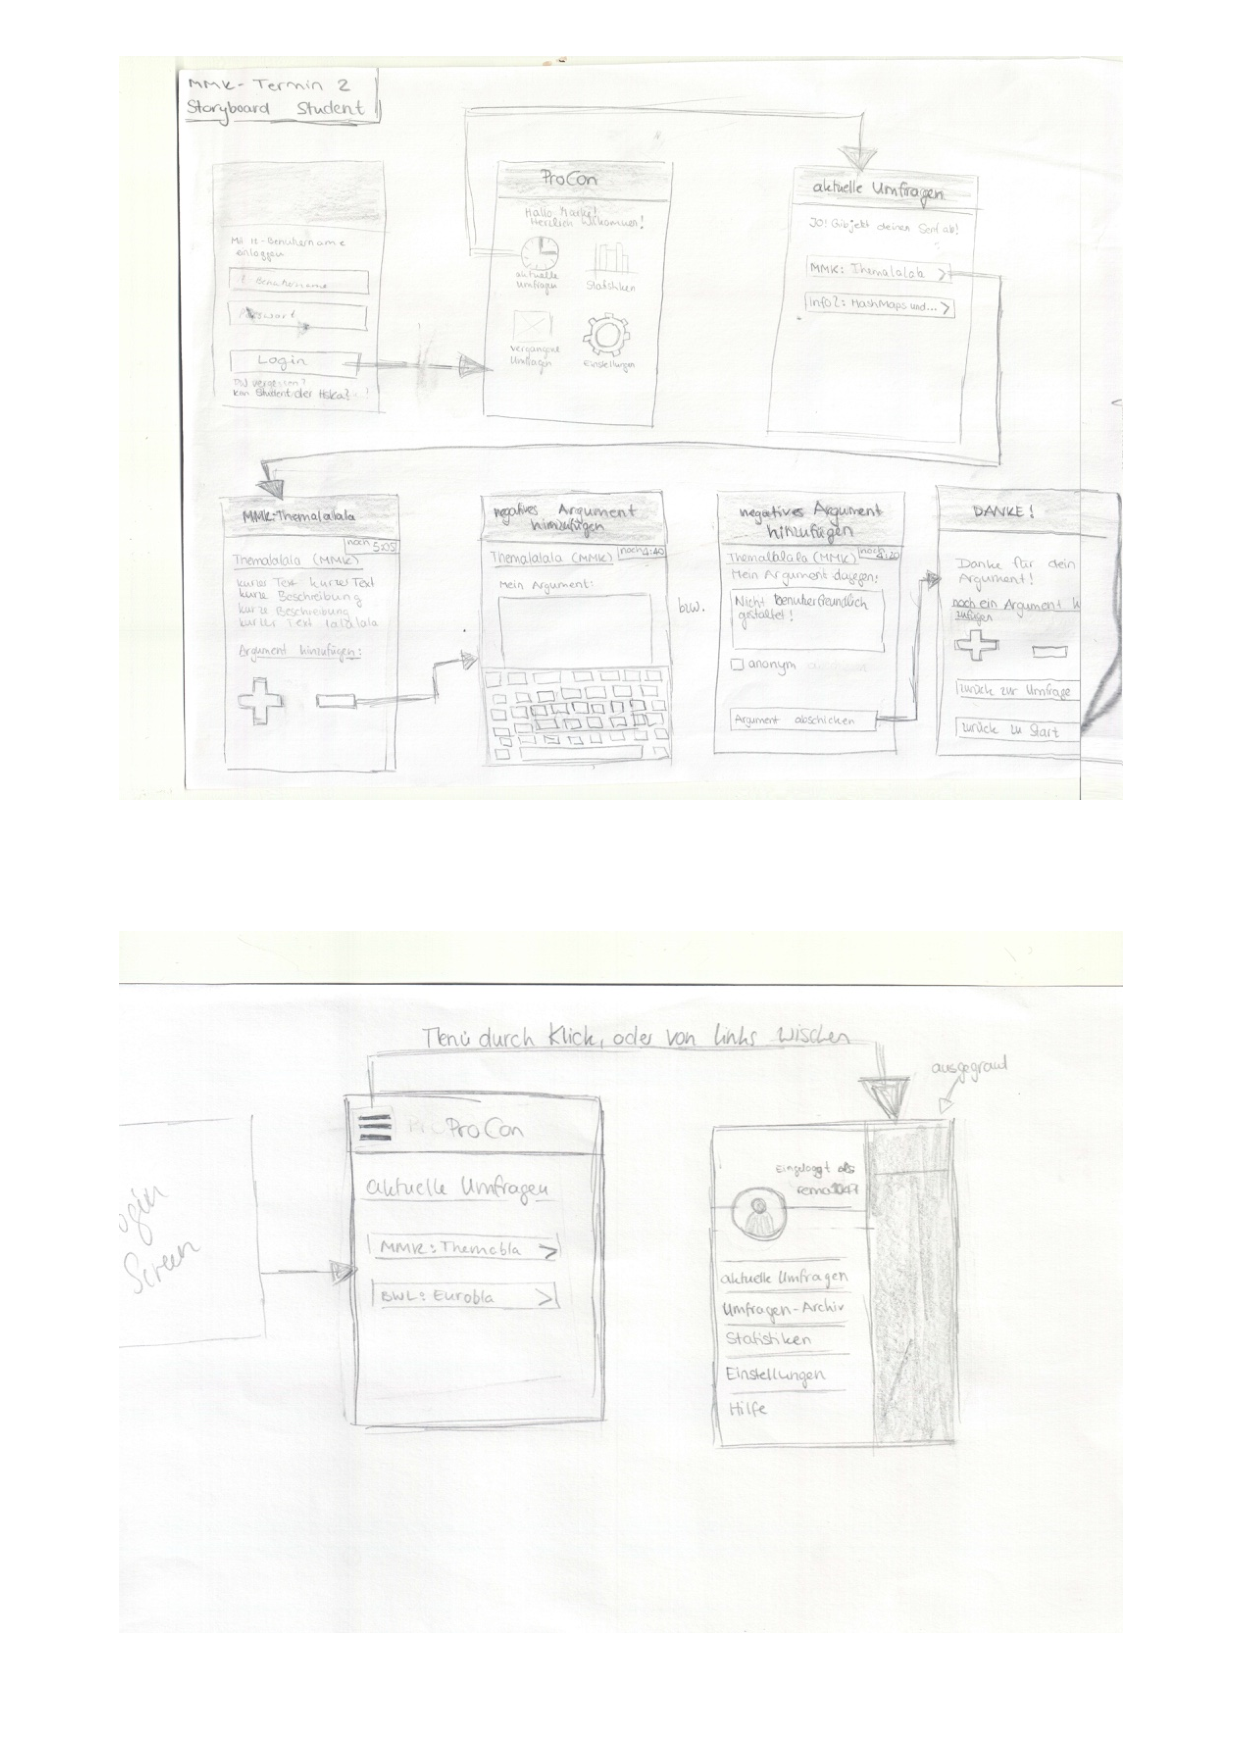
\includegraphics[page=1,width=0.85\textwidth]{./images/entwuerfe/maike}
  \end{center}
  \vspace{-40pt}
\end{wrapfigure}



\begin{wrapfigure}{L}{0.4\textwidth}
  \vspace{-20pt}
  \begin{center}
    \includegraphics[page=2,width=0.99\textwidth]{./images/entwuerfe/maike}
  \end{center}
  \vspace{-40pt}
\end{wrapfigure}



\begin{wrapfigure}{L}{0.4\textwidth}
  \vspace{-20pt}
  \begin{center}
    \includegraphics[page=3,width=0.99\textwidth]{./images/entwuerfe/maike}
  \end{center}
  \vspace{-40pt}
\end{wrapfigure}



\begin{wrapfigure}{L}{0.4\textwidth}
  \vspace{-20pt}
  \begin{center}
    \includegraphics[page=4,width=0.99\textwidth]{./images/entwuerfe/maike}
  \end{center}
  \vspace{-40pt}
\end{wrapfigure}

\clearpage



\section{Patrick König}
\label{sec:king}



\clearpage

\section{Tobias Kerst}
\label{sec:toby}

\begin{wrapfigure}{L}{0.4\textwidth}
  \vspace{-20pt}
  \begin{center}
    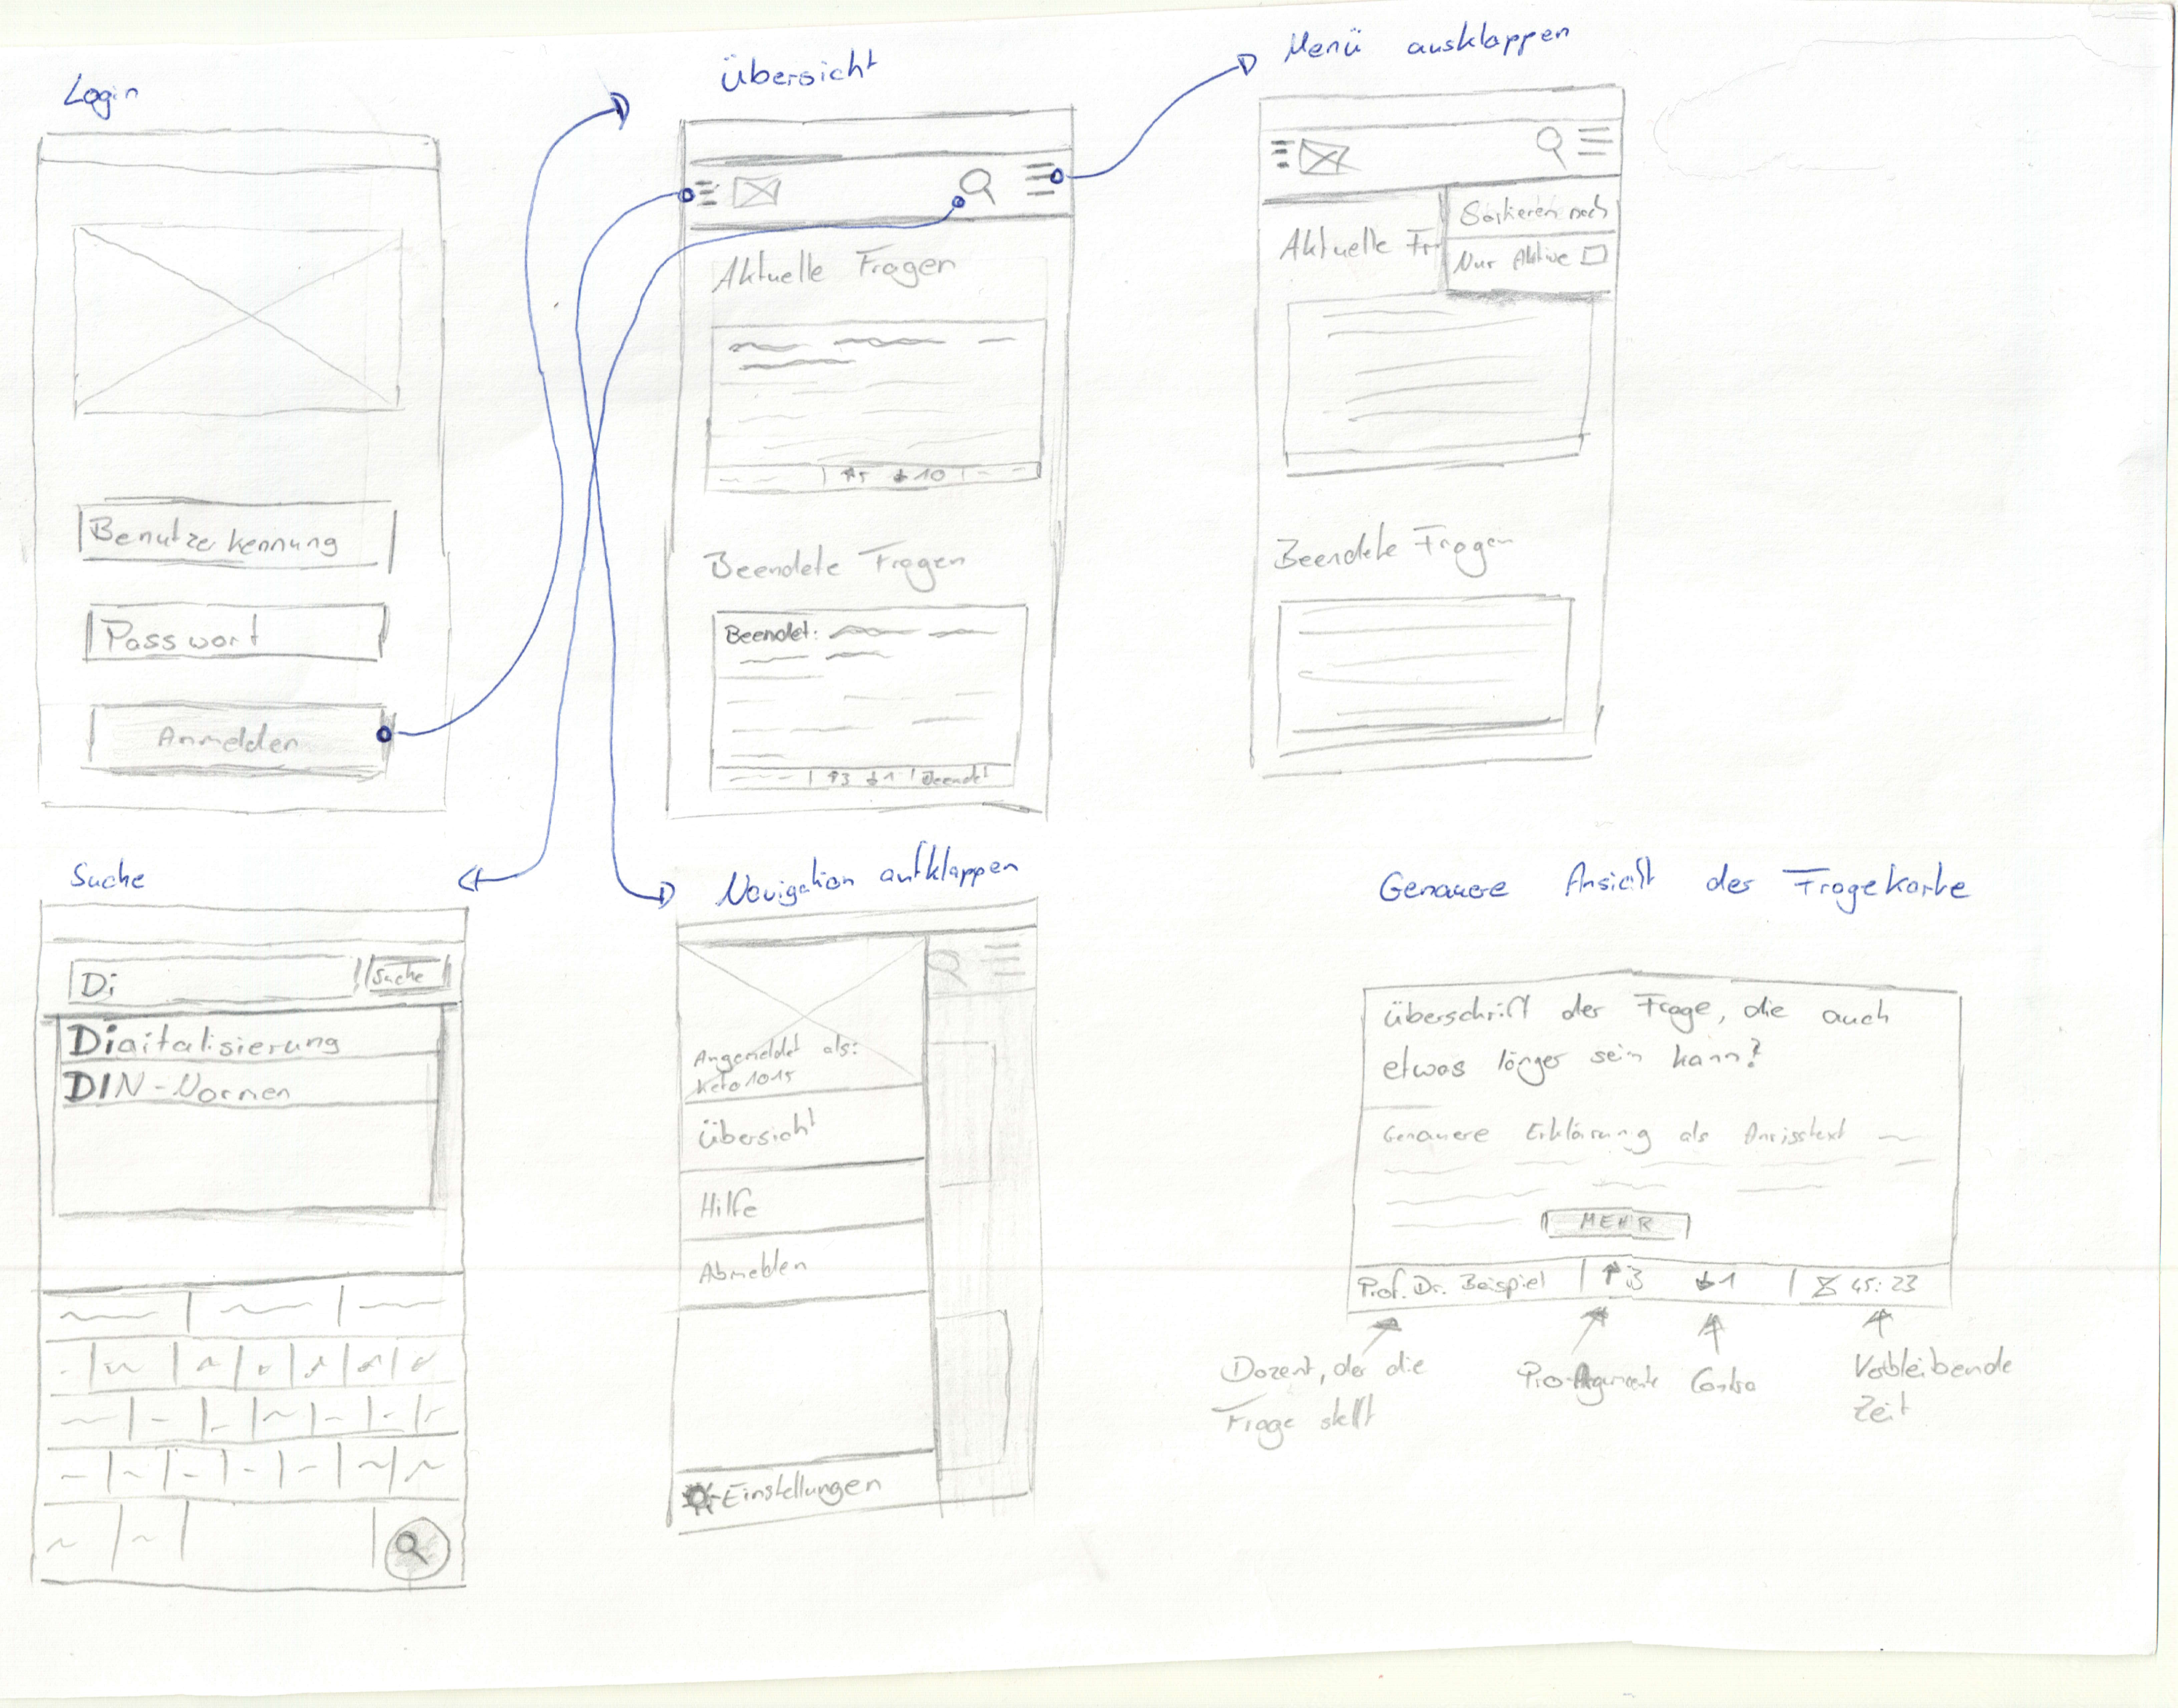
\includegraphics[width=0.99\textwidth]{./images/entwuerfe/toby1}
  \end{center}
  \vspace{-40pt}
\end{wrapfigure}

\clearpage
\begin{wrapfigure}{L}{0.4\textwidth}
  \vspace{-20pt}
  \begin{center}
    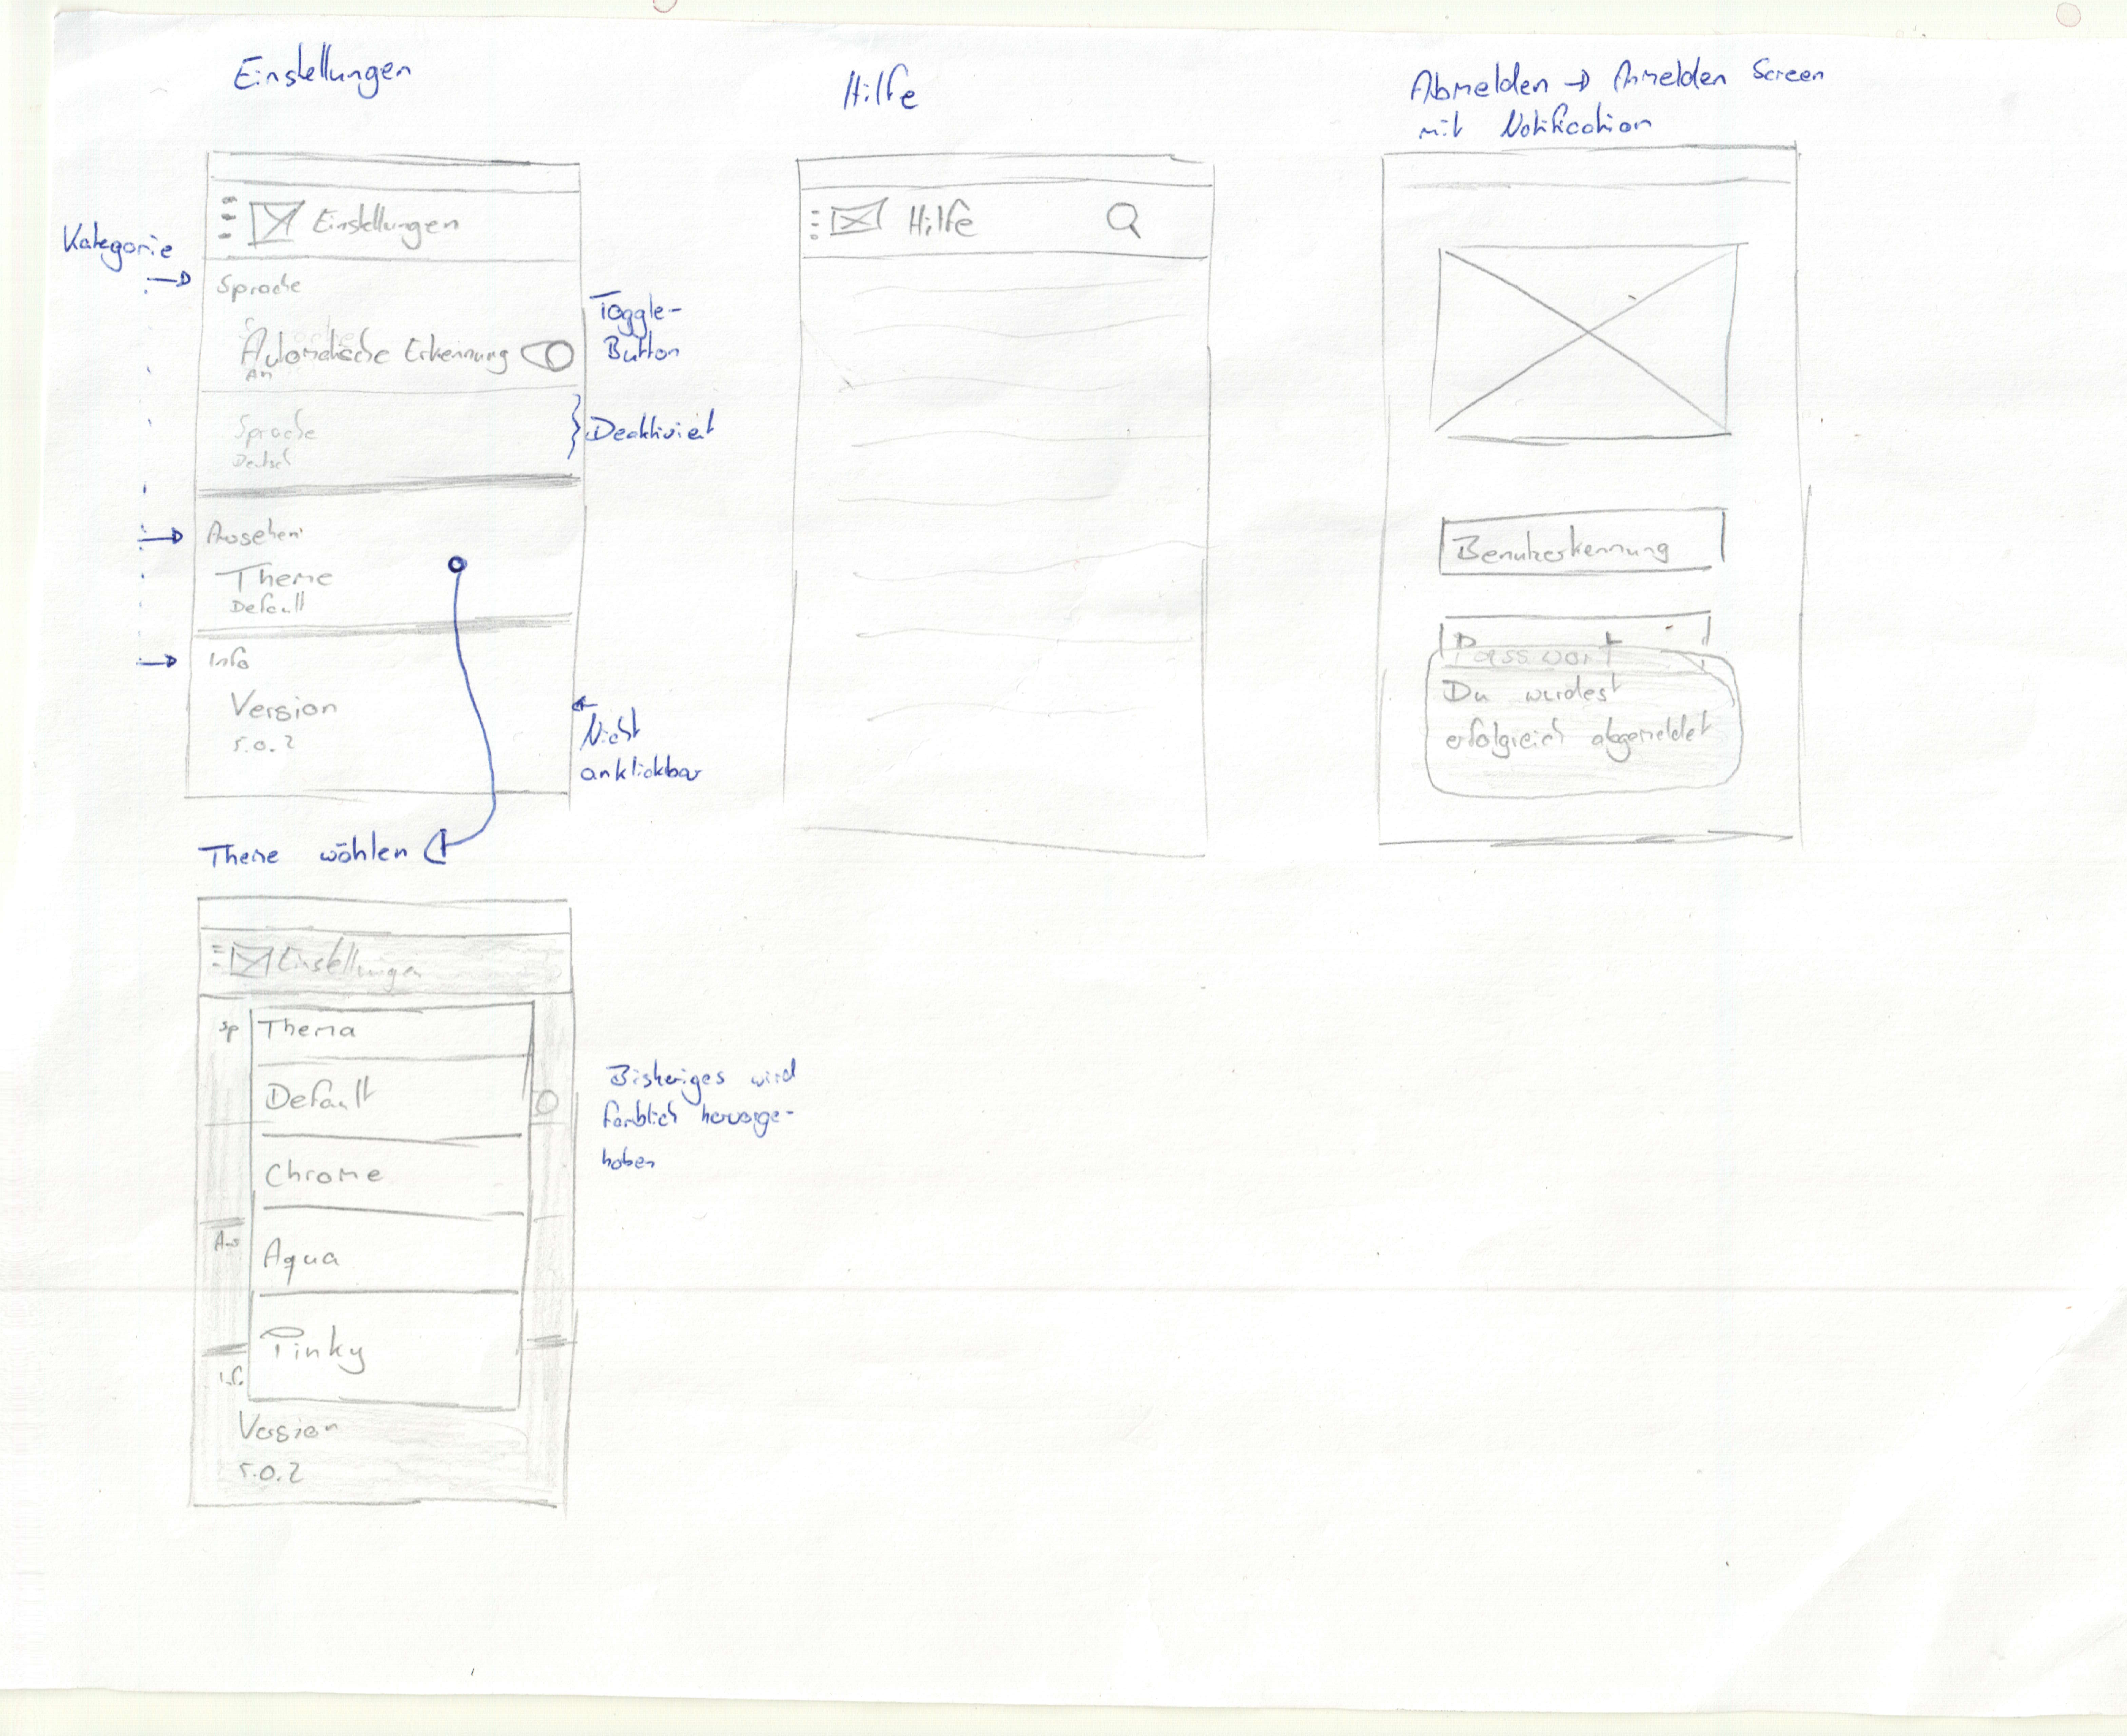
\includegraphics[width=0.99\textwidth]{./images/entwuerfe/toby2}
  \end{center}
  \vspace{-40pt}
\end{wrapfigure}


\clearpage
\begin{wrapfigure}{L}{0.4\textwidth}
  \vspace{-20pt}
  \begin{center}
    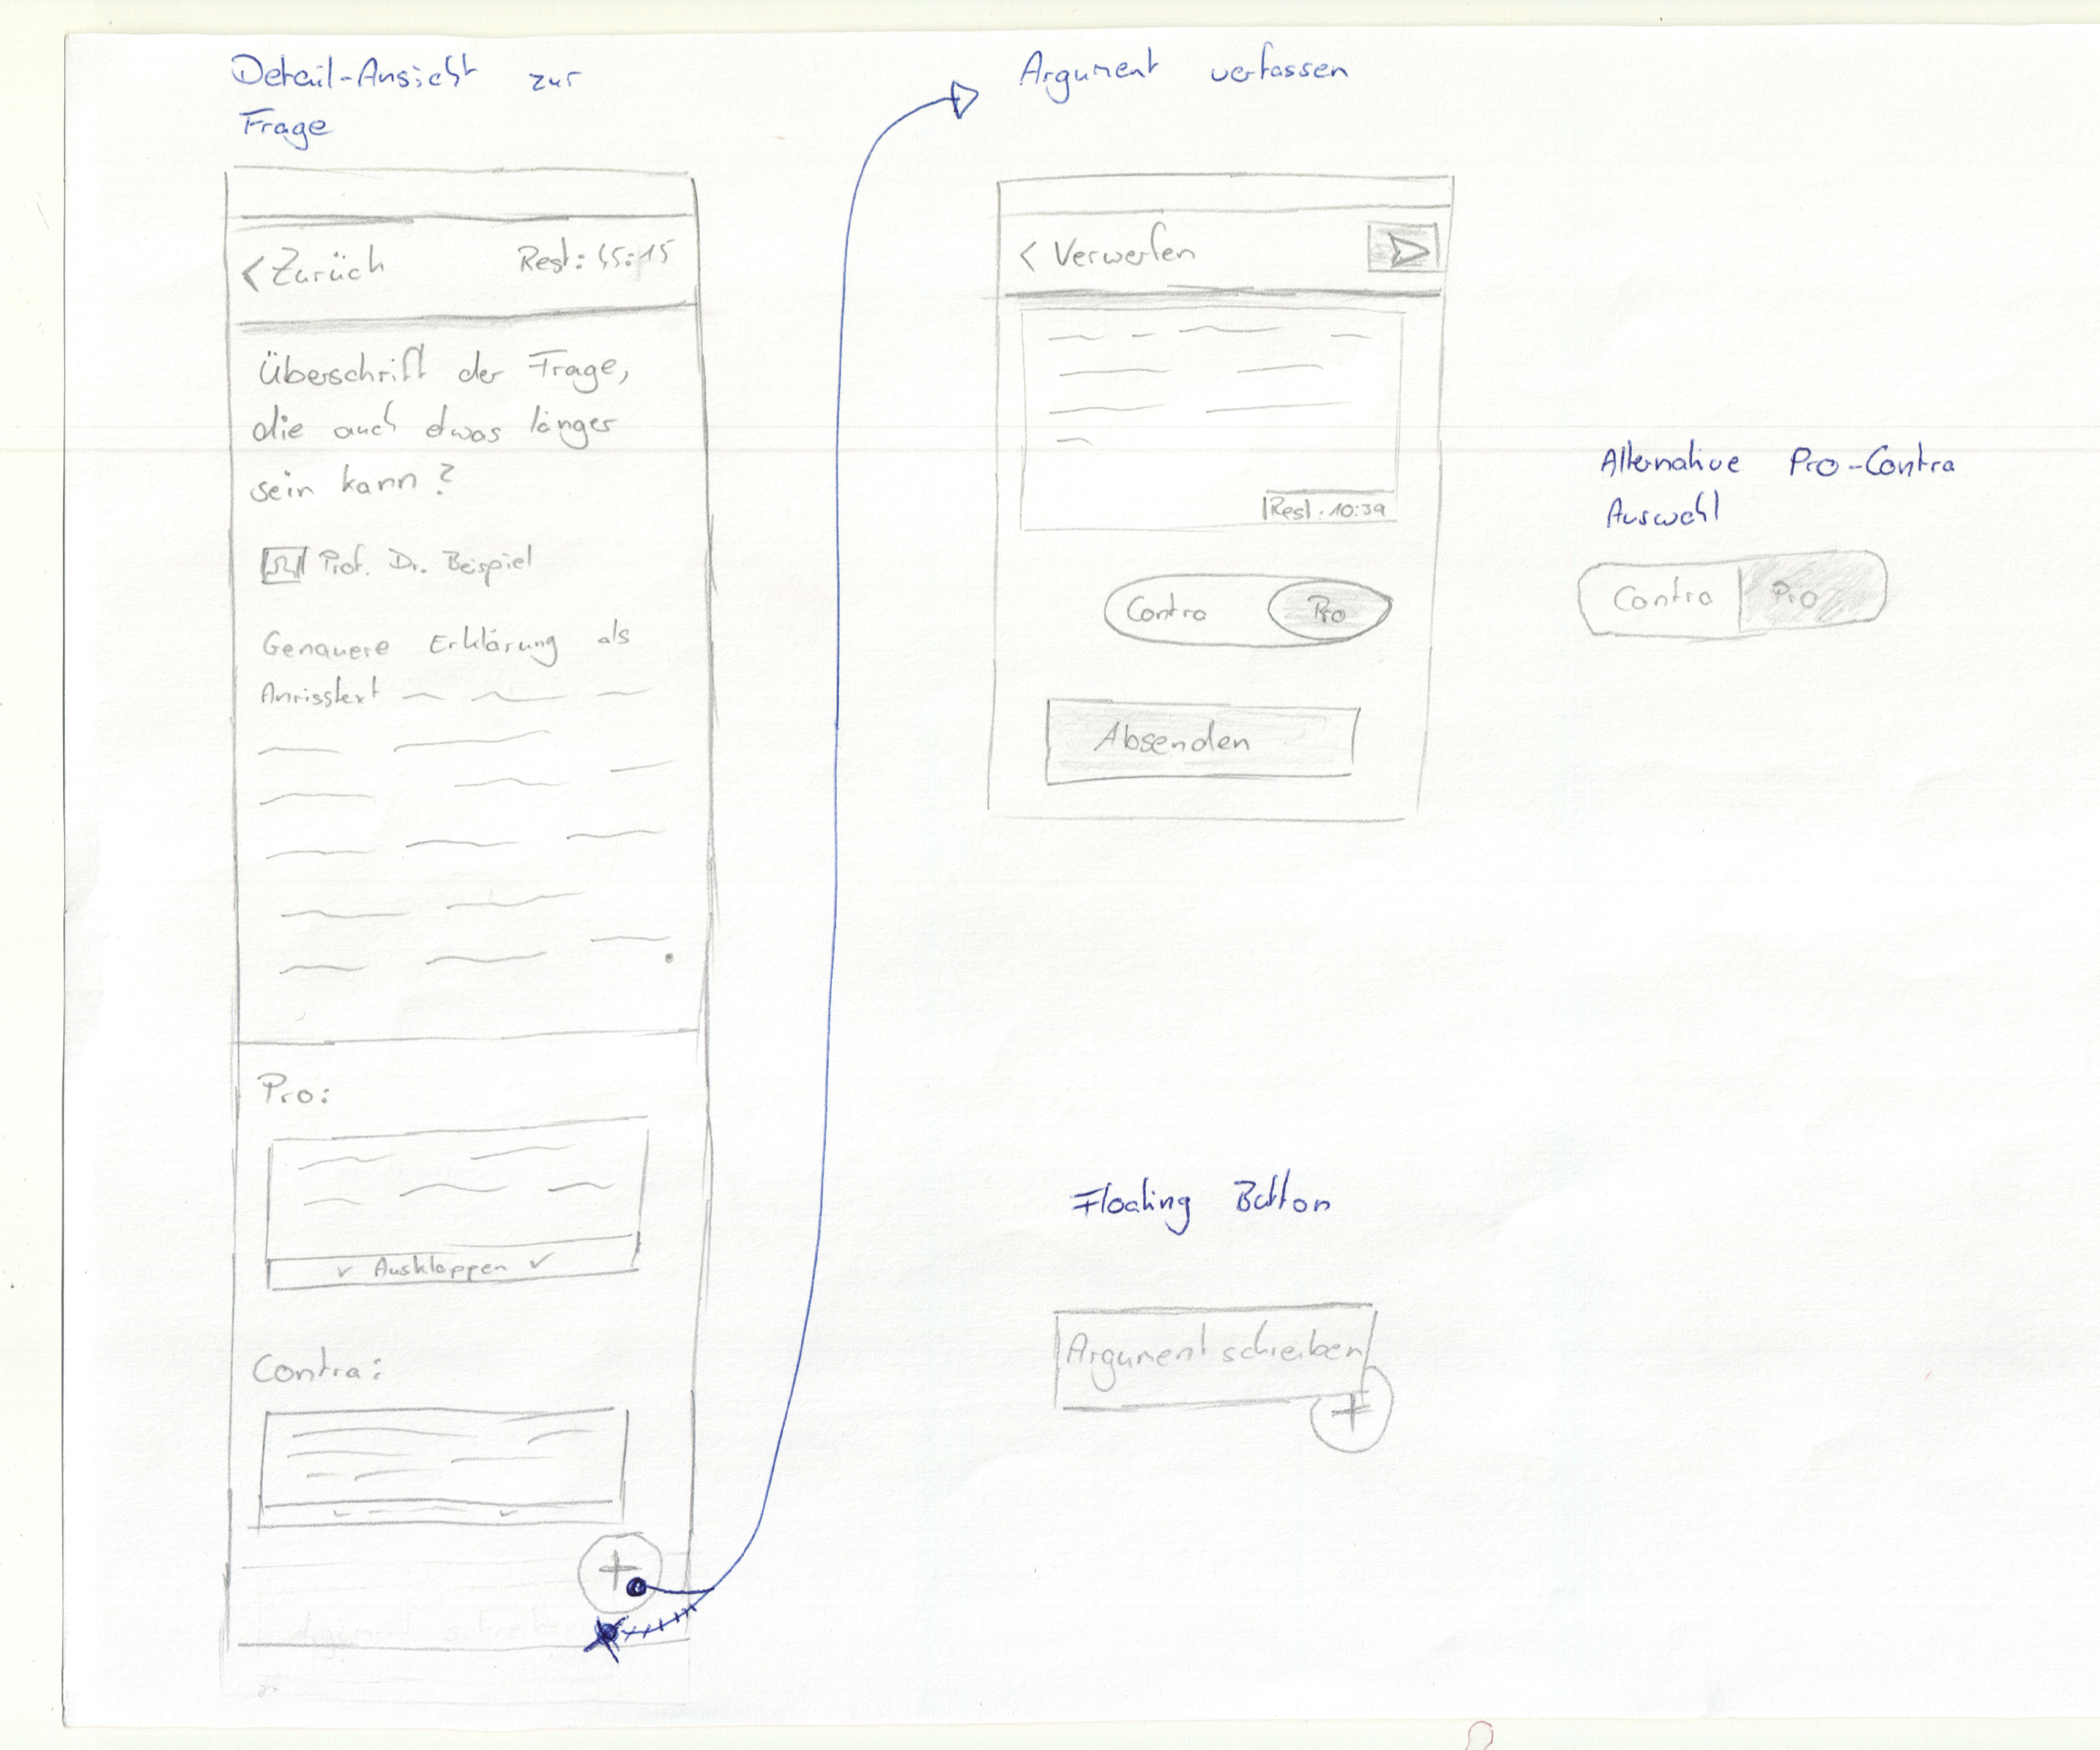
\includegraphics[width=0.99\textwidth]{./images/entwuerfe/toby3}
  \end{center}
  \vspace{-40pt}
\end{wrapfigure}


\clearpage

\section{Best of Storyboard}
\label{sec:bestof}

Das Best of Storyboard wurde anhand der Entwürfe von Maike und Tobias festgelegt und nur in kleinen Punkten geändert. Um Dopplungen zu vermeiden, verweisen wir hier auf die Prototypen in \ref{sec:prototypen}.

\subsection{Objekt-Hierarchie}
\label{sec:objekthierarchie}

\begin{wrapfigure}{L}{0.4\textwidth}
  \vspace{-20pt}
  \begin{center}
    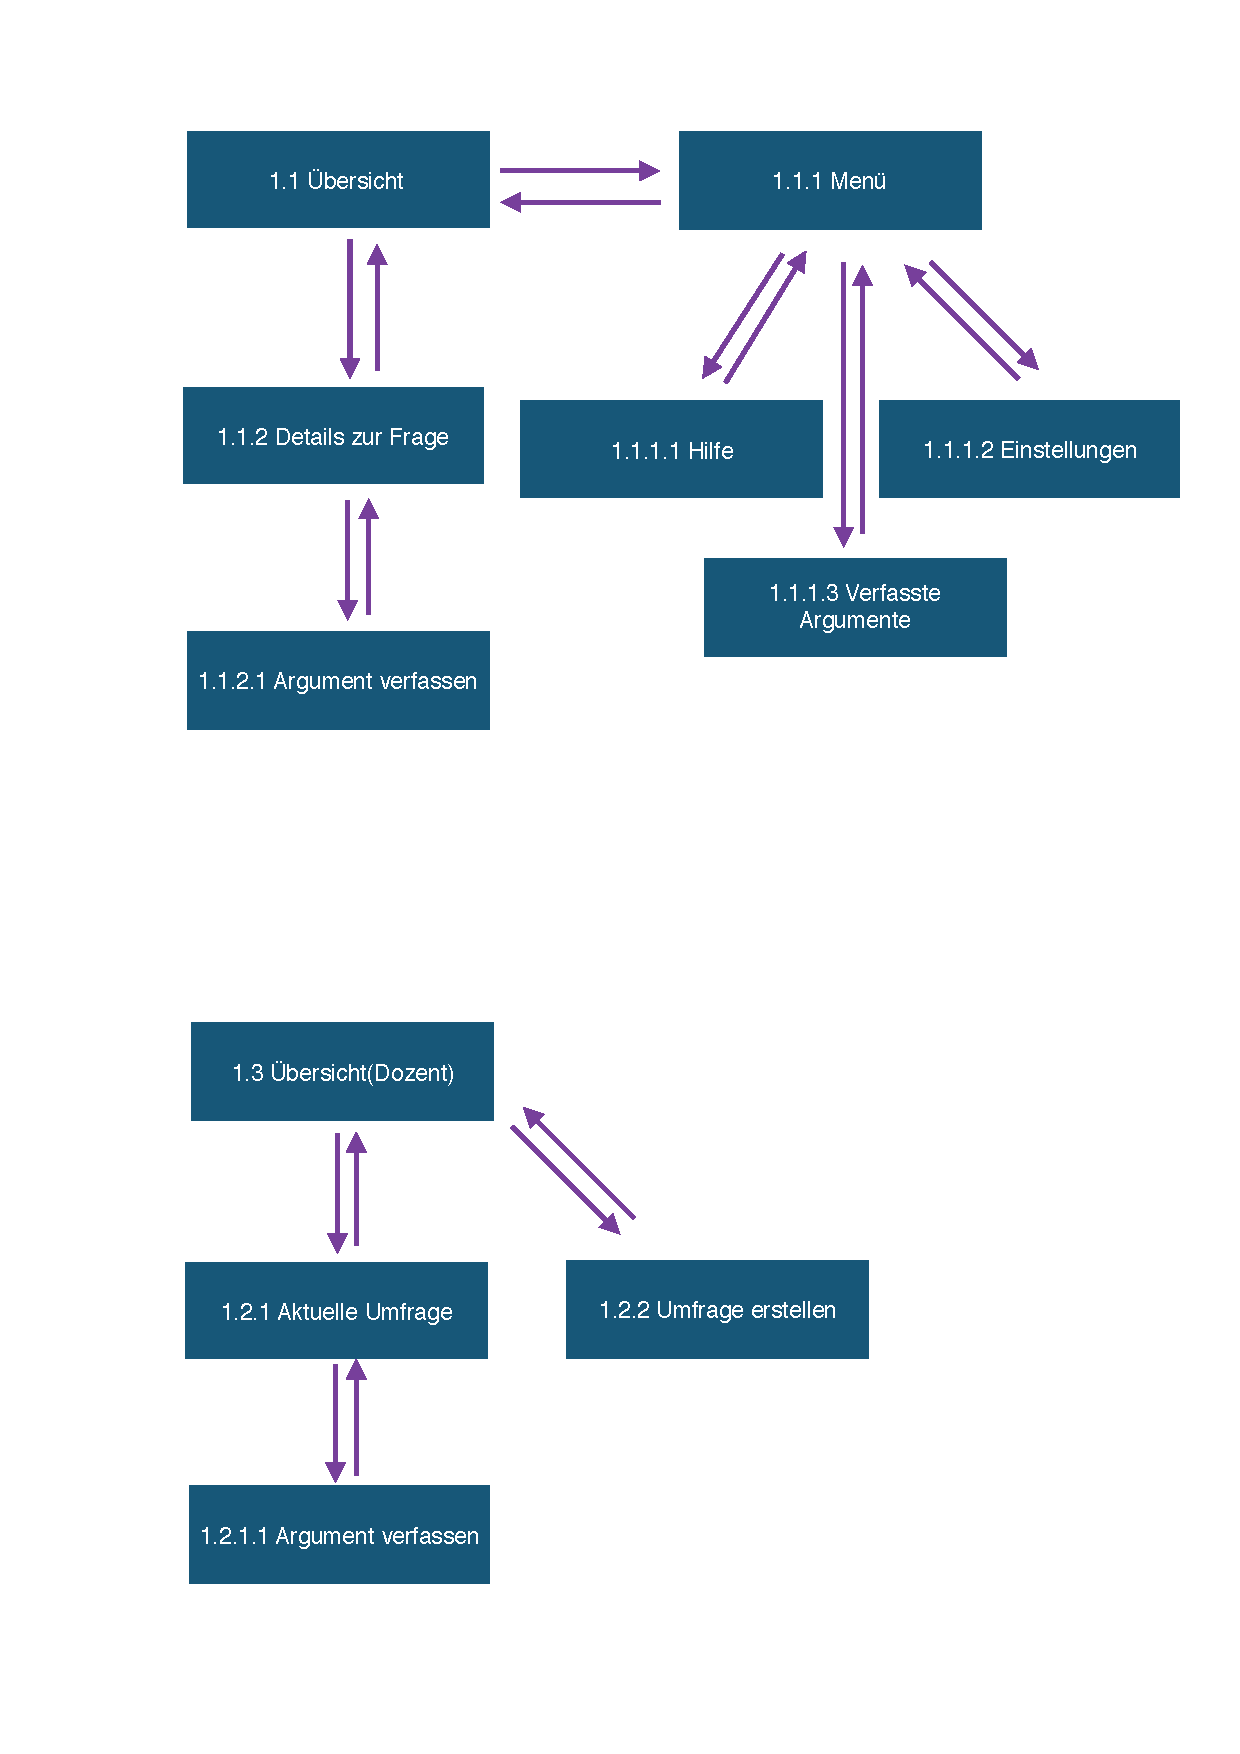
\includegraphics[page=1,width=0.79\textwidth]{./images/objekthierachie}
  \end{center}
  \vspace{-40pt}
\end{wrapfigure}

\clearpage
\subsection{Objekt-Attribut-Aktionen-Tabellen}
\label{sec:objektattribut}

\begin{tabular}{l p{5cm} p{5cm}}
Objekt & Attribute & Aktionen \\
\hline
Übersicht & Aktuelle Fragen, Beendete Fragen & Suchen, Navigieren\\
Menü & Navigationselemente & Navigieren\\
Hilfe & FAQ & Suchen\\
Einstellungen & Sprache, Info, Aussehen & Sprache ändern, Stil ändern, Theme wählen\\
Verfasste Argumente & Abgegebene Argumente & Umfrage aufrufen\\
Detailansicht zur Frage & Überschrift, Beschreibung, Dozent, Pro-Argumente, Kontra-Argumente & Neues Argument erstellen\\
Argument verfassen &Argument, Pro/Kontra & Absenden\\
\end{tabular}

\subsection{Tabelle der Bedienelemente}
\label{sec:bedienelemente}

\bgroup
\def\arraystretch{1.5}
\begin{tabular}{p{4.5cm} | p{1.8cm} p{2cm} p{2.5cm} p{2cm} p{1.8cm} p{2cm}}
Aktion/Attribute & Dedizierter Button & Seitenmenü & Ausklappbares Menü & Toolbar & Android Buttons\\
\hline
Suche &  &  &  & x & x\\
Argument erstellen & x &  &  &  & \\
Argument abschicken & x &  &  & x & \\
Argument verwerfen & x &  &  & x & x\\
Fragen sortieren &  &  & x &  & \\
Fragen nach Aktuellen filtern &  &  & x &  & \\
Einstellungen bearbeiten & x & x &  &  & \\
Hilfe abrufen &  & x &  &  & \\
Fragendetails ausblenden (Zurück zur Übersicht) & x &  &  &  & x\\
\end{tabular}
\egroup

\clearpage